\documentclass[final, dvipsnames, authoryear,12pt]{elsarticle}
\setcounter{page}{0} \renewcommand{\baselinestretch}{1.0}
\usepackage[utf8]{inputenc}
\usepackage{subfiles}
\usepackage{todonotes}
\usepackage[left=3cm, right=3cm, top=3cm]{geometry} 

\usepackage{epsfig,amssymb,calc,float,longtable,natbib,rotating,url, grffile, supertabular, subfig}

\setlength{\parindent}{0em}
\setlength{\parskip}{1em}

\usepackage{color}
\DeclareUnicodeCharacter{2212}{-}
\usepackage{blindtext}
\usepackage{mathtools}
\usepackage{mdframed}
\usepackage{graphicx}
\usepackage{caption}
\usepackage{subcaption}
\usepackage{enumerate}
\usepackage{hyphenat}
\usepackage[english]{babel}
\usepackage{colortbl}
\usepackage{amsmath}
\usepackage{booktabs}
\usepackage{multirow}
\usepackage{multicol}

\usepackage{changepage}

%font types
\usepackage{tgcursor}
\usepackage{courier}

\usepackage{tabularx}
\usepackage{tabulary}
\usepackage{threeparttable}
\usepackage{lscape}

\usepackage{bigstrut}
\usepackage{filecontents}
\usepackage{hhline}


\begin{document}


\begin{frontmatter}
\title{Global Value Chains localisation and firms competitiveness: Case studies on selected EU countries}






\author[gb]{G\'{a}bor B\'{e}k\'{e}s}
\author[mk]{Miklós Koren}
\author[bm]{Balázs Muraközy\corref{cor1}}
\author[at]{Álmos Telegdy}
 \address[gb]{Central European University, Institute of Economics and CEPR}
 \address[mk]{Central European University, Institute of Economics and CEPR}
 \address[bm]{University of Liverpool, Institute of Economics }
 \address[at]{National Bank of Hungary}
 
 
\cortext[cor1]{Corresponding author: Balazs Murakozy, xxxx } 

\cortext[cor2]{The authors gratefully }



\begin{abstract}
    Global....
\end{abstract}


\end{frontmatter}
%\maketitle

%%%%%%%%%%%%%%%%%%%%%%%%%%%%%%%%%%%%%%%
\section{Introduction}
%%%%%%%%%%%%%%%%%%%%%%%%%%%%%%%%%%%%%%%

The new wave of globalization in the 1990s brought about the formation of Global Value Chains (GVCs). These are companies linked by ownership and trade connections and are among the most important production structures of the global economy. The scale and importance of GVCs has multiplied during the last three decades.\footnote{\cite{mckinsey2019gvc}, for example, identify 23 GVCs and find that they account for 69 percent of global output and 96 percent of international trade.} Linking their countries' companies to GVCs is also high on the agenda of governments, as the integration into the production chains is among the most effective ways of improving competitiveness of firms and countries, and may also foster productivity and innovation.

Despite the attempts of governments to integrate national small and medium sized enterprises (SMEs) into GVC, we know surprisingly little about how connections in GVCs form. Lack of data prevents the study of buyer-supplier relationships in more detail. Existing empirical studies typically use industry-level measures to identify the trade between various countries' industries. More recently, firm-level information from administrative sources as well as survey data have also emerged. (In Section \ref{sec: approach} we discuss the advantages and disadvantages of various data sources.)

This paper describes our work in collecting both quantitative and qualitative information about buyer-supplier relationships in Hungary, Romania and Slovakia. After laying out our approach, we discuss the issues that arose during the data collection process. We also present a number of descriptive results about the structure of buyer-supplier portfolios of the firm, and how these are related to firm performance.

in terms of methodology: 
Presents a new approach which builds on a large scale survey linked to administrative data
Describes data collection and data handling in detail
Describes the issues such an exercise raises

In terms of substance
Describes key patterns in the data
Number, share etc of relationships
Geography of relationships
How relationships form
How the structure of relationships is associated with performance?
Can we identify high-value/key relationships from the data?



Administrative firm-to-firm data, such as VAT data, is scarce, and even if available, it is restricted to the amount of trade between firms, and do not provide much information on how the relationships develop and operate.

%%%%%%%%%%%%%%%%%%%%%%%%%%%%%%%%%%%%%%%
\section{Approaches to understand GVCs and supplier-buyer relationships} 
\label{sec: approach}
%%%%%%%%%%%%%%%%%%%%%%%%%%%%%%%%%%%%%%%

\subsection{Existing approaches and results}

To understand the importance of GVCs and their effect on countries, early research relied on industry-level input-output tables, constructed from international trade data (e.g., \cite{johnson2012accounting, hummels2001nature}. The main purpose of the use of such data were to (1) measure flows of trade between industries and countries and (2) compute the share of value added in gross exports. The data was also used to understand the propagation and amplification of small shocks in the economy (\cite{acemoglu2016networks}. The key finding based on aggregate data is that intermediate inputs played an ever increasing role in international trade since the 1970s, increasing abruptly in the 1990s. Certain limitations of this analysis, however, can be overcome only by using microdata.\footnote{For potential points of contact between the input-output and micro data approach as well as a concise treatment of the input-output approach, see \cite{johnson2018measuring}.} For example, the heterogeneity of firms by the number and other characteristics of business partners can only be studied in firm-level data. Interesting attributes of linkages include the number of upstream and downstream connections, the length of the relation, the type of firms connected to, among others. In addition, as input-output tables are typically based on import and export data, firm-level information is necessary to study intra-country firm connections, which is crucial for understanding which SMEs are able to connect to GVCs or large national enterprises.

An emerging literature studies business linkages and their effects on firm behavior. Two types of such data exist, those of administrative origin and surveys. \footnote{A common feature of all these data are that information on linkages and on firm performance (in form of balance sheet and income statement) are from different sources, and the performance data usually is of administrative origin.} 

Administrative data on business links is mainly derived from value added tax filings. \cite{dhyne2015belgian} covers Belgian companies (about 400 thousand firms). In addition to its great coverage, the data also follows firms in time (for 11 years). Papers using this data have studied the effects of international trade on firms costs (\cite{tintelnot2018trade}) and the sources of firm size heterogeneity (\cite{bernard2019production}). A limited set of business relationships are identifiable from Security and Exchange Commission filings of publicly listed firms in the U.S. \cite{Barrot2016-wc}. Shipments are recorded only if the buyer is a major partner of the supplier firm, defined as having at least 10 percent share in revenue. \cite{bernard2019production} build a model of outsourcing and test it on a Japanese database of the buyer-supplier relationships collected for credit risk analysis purposes. This data covers almost the whole Japanese private sector (800 thousand firms). 

URUGUAY?

ECUADOR?

A major survey on within-firm business relationships is the Commodity Flow Survey \cite{CFS}, which is based on a random sample of bills of lading for domestic and export shipments of U.S. firms. Even though the destination firm is not recorded on the survey, shipments are separated by ZIP code and hence internal within-firm shipments can be identified given the precise locations of firm establishments. \cite{atalay2014vertical} study the reasons for vertical integration of U.S. firms with the use two datasets: the Economic Census and the Commodity Flow Survey. These data are from 1993 (110 thousand establishments) and 1997 (60 thousand establishments). 

Among smaller-scale, more qualitative surveys, \cite{minetti2018financial} connects the effects of financial constraints on participation in local and global supply chains. The data are from about 7,500 Italian firms and have rich information on many aspects of firm behavior: the financial structure of the firm, including banking relationships, outsourcing, participation in supply chains and the propensity to innovate. \cite{newman2018linked}  uses data on 102 multinational enterprises and 226 domestically-owned firms from 5 African and 2 South Asian countries. The objective of this study is the measurement of knowledge spillovers of Foreign Direct Investment (FDI). In addition to the usual set of variables, the data have information on the ownership structure and R\&D activity.

The main advantage of administrative data is the larger sample coverage. As shown above, they usually cover most firms in an economy, if not the whole population. The large sample size sometimes is combined with information from multiple years, forming a panel. The information available, nonetheless, is rather limited and it is usually restricted to the existence of the trade link and the value exchanged. Survey data have much smaller coverage (a few hundred or several thousand firms) but they contain information on a special feature of the relationship or on firm behavior that is not present in the large datasets.

In our survey, we asked questions to understand the formation and quality of business ties between firms. According to our knowledge, no other dataset has such detailed information on business linkages. 

%% this theoretical discussion has little to do with data collection

%%% The closest to this question is perhaps the literature on how property rights shape the boundaries of the firm: which transactions take place within the boundaries of the (vertically integrated) firm and which on the market.\footnote{The theoretical and empirical aspects of this literature are summarized by \cite{antras2013grossman}}. Instead of firm boundaries, our survey focuses on market transactions and provide empirical evidence on their types and their effects on firm behavior.

Before describing the survey, it is useful to present the types of supplier-buyer relationship. \cite{gereffi2005governance} provide a typology of global value chains, which nevertheless can be applied to any type of supplier-buyer relation. The authors identify four types of trade relations between firms.\footnote{The 5\textsuperscript{th} relation is that of vertical integration, but we are interested in market transactions.}

\begin{description}
    \item[Market partners.] The commodity is simple and does not require any specific investment. Both the supplier and the buyer have many alternative partners. The cost of switching to a new partner is low for both the supplier and the buyer.
    \item[Modular partners.] The commodity is complex and it requires exchange of information between the two parties. The supplier can use general-purpose assets for the production and thus does not need the intervention of the buyer.
    \item[Relational partners.] The exchanged good is such that relationship-specific equipment is necessary to produce it efficiently, but both parties have a vested interest to maintain the relation (either because it would be hard to replace the partner, or due to some institutional arrangement, such as family ties between companies). Thus, none of the parties will hold up the other.\footnote{The hold up problem originates from the opportunistic behavior of some party in a relation (\cite{williamson2007economic}) and was introduced by \cite{grossman1986costs}. It consists of the expropriation of the other's investment value in a relationship which requires that one party invests such that the investment loses its value outside the relation.}
    \item[Captive partners.] In this relation not only relationship-specific investment is necessary, but one of the parties is able to extract part of the value of this investment. The reason for this can be, for example, the sheer size difference of the parties. For example, small local suppliers can be completely dependent on large international buyers and thus have not much bargaining power in the relation.
\end{description}

As can be seen from the typology, the relation between two firms may lie between a simple market relation and a strong bound of interdependence. The type of relation is shaped predominantly by the specificity of the product exchanged. To obtain an intermediate good that is simple does not require the development of a special relationship with its producer as it can be simply procured from the market, even if it is of crucial importance in the final product.\footnote{Note that if the timing of the arrival of the product is crucial even a simple intermediate good may become specific.} The supplier-buyer relation with exchange of specific intermediate goods will depend on two factors: whether there is need for a specific investment to produce the good and whether there are multiple buyers or suppliers of the good (and hence how competitive the market is). If there in no need for a relation-specific investment, the relation will be modular and only information will be exchanged between the parties. If the relation involves asset specificity but both the supplier and the buyer are the only ones who produce and need the product, the relationship will be relational.\footnote{This is similar to firm-specific human capital of workers. If a worker has to develop skills that are costly and she cannot use in other firms, the cost of this human capital investment should be shared between the employer and the employee so both have a vested interest in maintaining the employment relation (\cite{becker1962investment}.} At the opposite end from market transaction of the relational spectrum lies the situation when the supplier has to make a relationship-specific investment but the buyer has the opportunity to replace the supplier (for example, the buyer is a large multinational and the supplier a small domestic firm).  
    
In the following we present our survey methodology and discuss that specific questions that are meant to elicit information from the firms for the purpose to study the type of market transaction.
  
\subsection{Our aim and approach}

In the existing literature, relatively little is known about how linkages form between firms. Our aim was to design a method which would be informative along this dimension. It is of interest to collect basic information about business partners, such as counting buyers and suppliers. However, such basic data is provides only a limited amount on information on how relationships form an operate and we decided to collected further information on how relationships are formed and maintained. To keep the survey of a managable length, we asked these questions about a limited set of business partners. The literature suggests that both firm fundamentals (productivity, size, etc) and strategic choices matter. Because of this quantitative data on links and administrative balance sheet data strongly complement each other. We hence asked firms to name their business partners so that we can merge their balance sheet data.

%%%%%%%%%%%%%%%%%%%%%%%%%%%%%%%%%%%%%%%
\section{ Survey}
%%%%%%%%%%%%%%%%%%%%%%%%%%%%%%%%%%%%%%%
\subsection{How it started}

% todo gabor. 

\begin{itemize}
    \item Idea
    \item Team: background, experience with firm data, surveys, microdata management
    \item Choosing GFK as partner
\end{itemize}{}


\subsection{Designing the survey instrument}

Although more and well detailed administrative datasets are available about companies, some concepts and organizational practices are still badly measured.\cite{Bloom2014-hc} One of them is the way firms form and maintain relationships. This topic is rarely analyzed with empirical techniques, even though it is potentially related to firm performance. Our survey focuses on supplier-buyer relations and analyzes how these choices influence the firms’ development.

We first sketched all possible topics for the survey based on our review of the economics and business literature. 
Some of the questions were original and some of them were imported from already existing surveys (e.g. from the EU standard Community Innovation Survey). It was clear from the beginning that the survey should be formulated in a way to maximize response rate. Therefore we discussed the methods and topics covered with colleagues from our survey partner and also with industry participants.

Based on the expert judgment of our survey partner, we decided that the survey will last no longer than 45 minutes. Given the breadth of topics we wanted to include, this meant significantly length constraints on our questionnaire. The other important feedback we received reflected on the methodology. We decided to restrict the number of open ended questions and mainly included multiple choice or close ended (yes or no) questions. An important exception was asking the managers to briefly describe their firms, as this may contain useful information that helps to understand the context of their answers. These small bits of information capture the reasons behind altering answers. For example big changes can be explained by opening to foreign markets or the structure of partnerships can be better understood by knowing that the firm only buys from and produces to its parent company.

An important aspect of the survey was to discover the criteria system firms use when selecting their potential partners. We listed some possible options (price, flexibility, reliability, quality of the products, etc.), but in our pilot studies we found that respondents marked all of them. The interviewed managers considered each of them an important aspect, and the way we formulated the question did not help to put them in order of importance. Therefore we started to experiment with different methods to identify the most important characteristics. We asked the firms to rank them or to compare to other options on the market to find the best methodology.

We wanted to identify as many suppliers and buyers as possible and also collect detailed information about them (such as location, ownership, products sold and also relationship specific information such as the length of cooperation, the first steps in establishing relationship, assistance received from the partner). This posed a trade-off in the number of partners asked about and the brevity of the survey. We decided to ask details only about the partners that have a higher than 10\% share in sales/material costs or the three most important ones. This definition worked very well and firms could easily identify their partners. We also included a section about a special supplier/buyer the respondent wants to mention, even if they were not among the largest partners. Such special partner can be the oldest partner, a firm that is a good reference, or a foreign partner.

To choose the most important topics and related questions and also to avoid asking about confidential information we met with industry participants. With their cooperation we ran three primary interviews about their firms. During these interviews we learned a lot about what topics to cover and how to ask the right questions. It was extremely helpful as asking the right questions can have a positive impact on response rate as well. As researchers it is sometimes hard to understand the day-to-day operation of firms and we had a chance to see the important aspects that create differences between business groups. We learned about different ways of establishing partnership that we have not thought before. One of them was meeting at an expo, which came up many times later on. It also became clear that we need a clear strategy to ask the relevant info for corporate groups. Especially in the case of big companies firms are strongly connected within a corporate group. In their case many of the original questions lost relevance so we had to include an option to distinguish these companies from independent ones.

We dropped all the questions that have answers available in other datasets and only included some financial numbers (total and export revenue) to help identifying firms and some information not available otherwise (distinction between full-time and temporary work force). Suggested by Bloom, Lemons, Sadun, Scur and Van Reenen (2014) asking about financial situation decreases response rate as it is a confidential information and also because it requires some effort to get the exact numbers. Our experience was in line with that as managers of small companies claimed that only the accountant knows the exact values. So we could not receive the information from him.

\subsection{Finding the right terms and formulating the actual questions}

Another challenge we faced was the different jargon used by researchers and industry participants. As this could lead to serious misinterpretation which would later screw the results, we applied the modifications suggested by them. To understand the key terms used in this field, we attended at the 2015 Supplier Conference. The aim of the conference was to provide help for companies to become global by joining value chains. It showed some forums where the companies can meet and know each other and there were many presentations about the requirements a supplier should fulfill. This event was a great help in understanding the different roles a firm can play in a value chain (e.g. based on the nature of products supplied), the most important challenges they face (for example we got a deep understanding of the audit process before receiving ISO certificate) and the reasons firms opt to have foreign partners instead of Hungarians. This was a critical step in the evolution of the questionnaire and implied serious modifications to make it more life-like. Later it turned out that some of the participants still evaluated it too theoretical.

Identifying the exact partners is essential to create a network of buyers and suppliers. To maximize the accuracy of data we asked the firms to provide the EU VAT number of their partners. We needed it to merge the information with Amadeus dataset for further analysis involving financial data. It turned out that company name is not enough to identify partners in Amadeus, especially for foreign firms. As this information is usually not available on the spot we decided to provide an opportunity to later extend the information provided. The first interviews suggested that firms do not want to bother with looking for the EU VAT number and we got very bad coverage here. It was also clear that they are not keen on looking for this information after the interview is done.

It was a huge challenge to find the right questions about the topic of branding in the manufacturing sectors. Many of our pilot partners do not use it in a way we thought. They e.g. use identifiers to mark their products which is especially useful if maintenance is needed. However according to our research questions it should not be considered as branding.

\subsection{Definitions and a multi-language mindset}

After the first version of the questionnaire was ready we conducted five pilot interviews together with Gfk. Figuring out a questionnaire is not enough, we also had to construct it in a way that the interviewers are able to fill them. Since our survey requires some degree of business knowledge and is an interactive conversation we asked our partner to hire skilled interviewers. On the top of that after deriving the conclusions from the pilot version we organized a training where interviewers had a chance to understand the questions in depth and discuss their worries with the organizer team. Similar events were later organized in each participant countries. Definitions were explained to the interviewers to have comparable data. For example it makes a huge difference whether they give the share of supplier compared to sales or EBITDA. All the interviewers needed to be confident in using these business terms.

It was very important to make a hub in each participating countries and provide a chance for the managers to answer in their native language. We also ensured the possibility that if nobody from the management speaks the native language of the country than the interview can be done in English with the support of skilled individuals hired from the field of economics.

\subsection{Building trust}

Response rates to surveys have been falling over time \cite{Bloom2014-hc}. This finding was reinforced by our experience. Managers claimed that they receive more than one survey call a week therefore we had the challenge to make the survey attractive. We applied many different approaches.

We promised the participants an analytic report and industry level summary from the results. These outputs can help them to understand the general trends in their industry and compare their firms to industry averages. Naturally all published/distributed results are carefully anonymized (see below).

The survey was managed by respected institutions (Central European University and the Institute of Economics of the Hungarian Academy of Sciences) and also received professional support from other associations (such as the Hungarian Association of Logistics, the Slovak Economic Association and the Faculty of Economics and Business of Babeș-Bolyai University). Funding for the survey was provided by the European Research Council and the Lendület Program of the Hungarian Academy of Sciences. These associations were kindly asked to boost response rate among their members by introducing the survey to them.

To market the survey, we created a website, suppliersurvey.eu, available in four languages: English, Hungarian, Romanian, and Slovak. We advertised the survey on related business events, such as the Figyelő forum, which is one of the most prestigious business magazine in Hungary. Communication was also extremely important when we contacted the firms. We put a lot of efforts in writing a letter of introduction that describes in a clear language the ways we are going to use the dataset.

Another issue was to find the appropriate person in the firms. It was not always clear who has all the information that we needed. Our questionnaire required information about supply, which could have implied that the target person is the Procurement Officer. However, in many cases partnership decisions require higher level acceptance. The questions are related to strategic decisions and sometimes has a strong impact of the general operation of the firm. For example joining a global value chain requires many ISO certificate that implies the revision of the entire operation and adoption to pre-defined standards at many levels. It was the responsibility of the interviewers to find the right person within the company. (We collected the position of the interviewee to check for differences based on that.) The position of the interviewed person with the identity of interviewer was collected to improve precision of the estimation.

\subsection{Sampling choice}
We constructed a sampling frame based on the AMADEUS database (\cite{amadeus}) so that we can link survey responses to financial information. The target population included manufacturing firms in the industries between 20 and 30 (NACE Revision 2) with at least 10 employees.

We selected firms for which basic financial information for 2012 and 2013 was available. We anticipated a response rate of 30\%, so our sampling frame included more firms than the actual sample. We used two dimensions of interest in the sampling stratification strategy: size (10-50, 50-250 and over 250 employees) and ownership. We only distinguished foreign and domestic firms, where all companies with at least one non-Hungarian owner were considered  foreign. Both variables came from the Amadeus dataset. We created inverse probability weights to restore the representativity of our sample to the whole population of firms in the target population.

Our survey partner received basic identifying information for each firm in our sampling frame (name, industry, address of the headquarters), randomly ordered within each stratum. They were also given target numbers to reach, separately for each stratum. These targets implied oversampling of smaller hard-to-reach groups like large foreign firms. The size of the sample from the three participating countries were adjusted according to their population. Slovakia had 500 firms, Hungary had 600 firms and Romania had 700 firms.

Table \ref{} reports the sampling probability for each stratum, calculated as the number of firms in the final sample divided by the number of such firms in the target population.

% todo gergo: create this table. if you don't have original amadeus data used to create sampling frame, use sampling frame only and edit language "target population" -> "sampling frame".

Given our sampling frame, we could link our survey data with Amadeus, adding financial information such as sales or assets. At this stage, all financial variables refer to 2013. Eventually we have financial information (such as total sales in 2013) for 82\% of firms in the sample. 
% TODO: Gergő check all numbers reported

\subsection{Pilots}
We did 10 pilot studies in two rounds, testing two versions of questionnaire. We picked large companies as well as SMEs, domestically and foreign owned as well. Pilots were essential in deciding about the final version of the questions. Based on feedback from the pilot, we simplified some questions. For example, we merged several possible answers, as managers had a broad idea about the industry of the partner, but not much detail. We also added some explanations to questions and answers to make sure respondents understand the questions equally well. This was especially important for questions on innovation and learning. 

\subsection{Questionnaire}

Some questions on all suppliers/buyers in a symmetric fashion. 

%%%%%%%%%% TABLE Q1
% TODO Gergo
ADD: Table here with example questions
basically two columns, Q for buyers and Q for suppliers, about 5-8 questions
+ response rate for each q

%%%%%%%%%% TABLE Q2
% TODO Gergo
ADD: Table here with example questions

More detailed question on a subset of suppliers/buyers 

basically two columns, Q for buyers and Q for suppliers, about 4-5 questions
+ response rate for each q

%%%%%%%%%% TABLE Q3
% TODO Gergo
ADD: Table here with example questions

We also added questions asking about the supplier / buyer pool. 

basically two columns, Q for buyers and Q for suppliers, about 2-4 questions
+ response rate for each q


%%%%%%%%%% TABLE Q4
% TODO Gergo

ADD table on machines
column 1: questions similar to buyer/supplier
column 2: machine specific questions
+ response rate for each q


%%%%%%%%%% TABLE Q5
% TODO Gergo
ADD table on general questions
Questions on firms, like employment
+ response rate for each q

\subsection{Survey Method}
% todo gabor

computer assisted personal interview

cannot randomize surveyors across respondents

not as much room for surveyor subjective interpretation as in WMS

% todo gergo
report some surveyor fixed effects

%%%%%%%%%%%%%%%%%%%%%%%%%%%%%%%%%%%%%%%
\section{Data handling and cleaning}
%%%%%%%%%%%%%%%%%%%%%%%%%%%%%%%%%%%%%%%

We created process where we create a file to describe the data structure, and transform raw data into data suitable for analysis. Figure \ref{fig:ERD} illustrate the logical model of our dataset in an Entity-Relation Diagram.

\begin{figure}[!h]
    \caption{Logical Model of the Supplier Survey Dataset}
    \label{fig:ERD} 
    \begin{center}    
    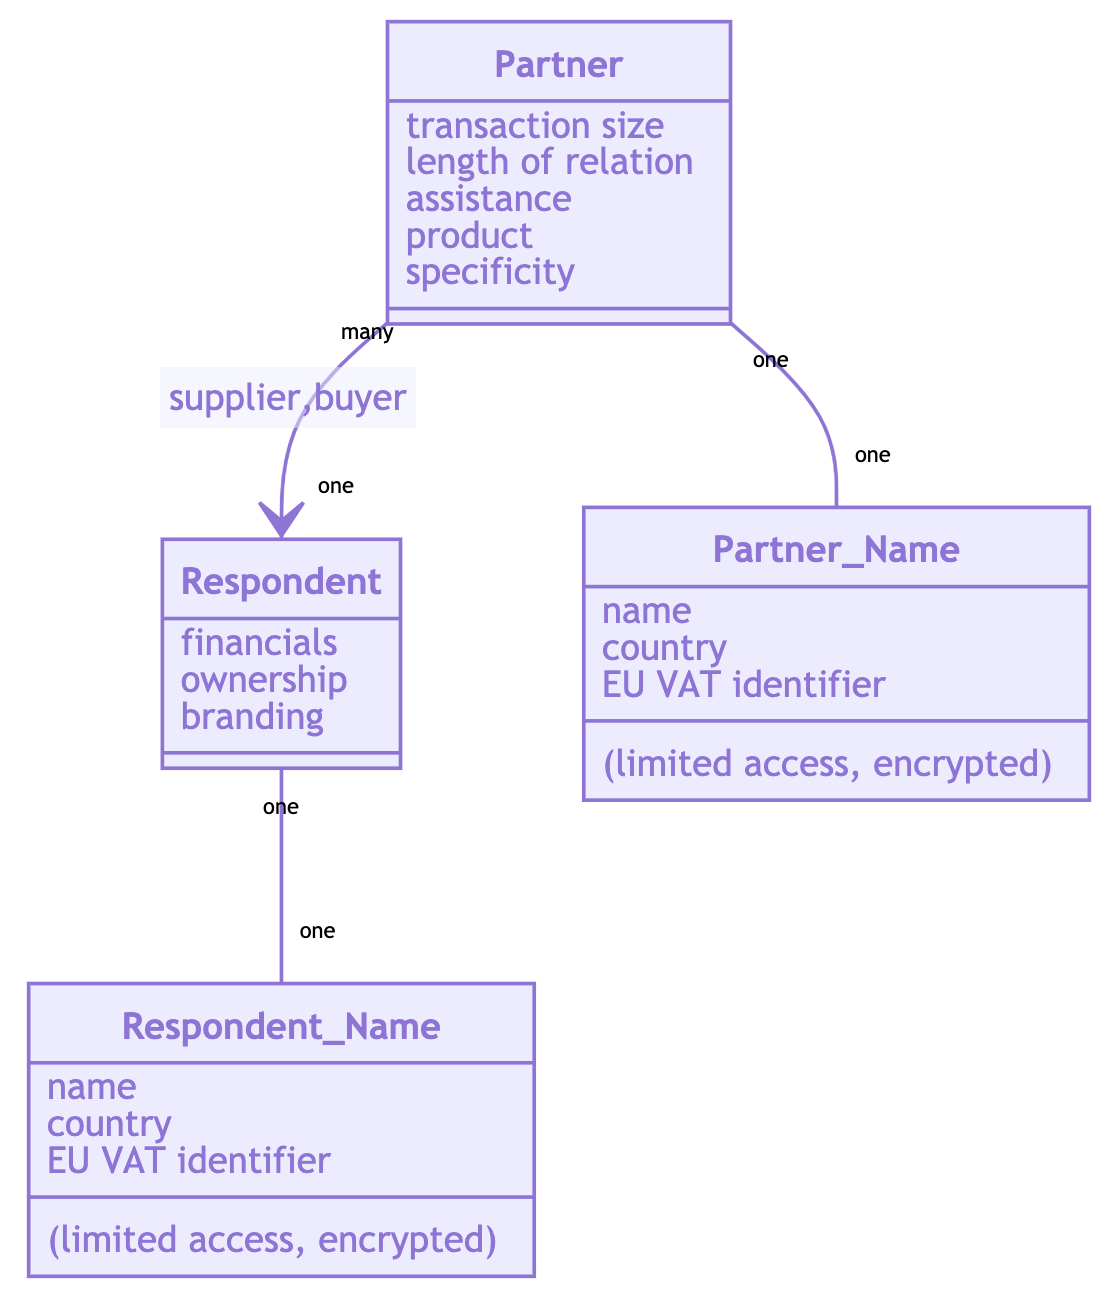
\includegraphics[width=0.7\textwidth]{graphs/ERD.png}
     \end{center}    
        {\footnotesize \textit{Notes:} This Figure shows the Entity-Relation Diagram of our analysis dataset. Each respondent can have multiple partners reported. The names of respondents and partners have been separated out in tables and handled separately to preserve anonymity. The graph gives a sample of information know about each entity, not a full list of variables.} 
\end{figure}

\subsection{Anonymization and data storage} 
As we asked about very confidential information that are in the core of an organization’s strategy, our data handling policy was an important issue from the very beginning. We consulted with lawyers about legal constraints and also with industry participants to understand their needs. Our research was also approved by the Ethical Research Committee of Central European University and underwent an ethics self-review for the European Research Council.

We formulated a Data Security Policy that is acceptable for each party and ensures data protection (see Appendix ??). It contains the exact details about what kind of data is collected for what purposes, and the technical and personnel restrictions on data access. These assurances notwithstanding, some of the interviewees refused to reveal private, business sensitive information such as the name of business partners. Among the ?? respondents ?? did not name any of its business partners.

Our data workflow provided a robust approach to anonymization. In particular, all information on company names and other identifiable information were masked, and even researchers could only work with data with anonymized  information only. In addition, we checked variables and cleared names from text (sometimes firm names were mentioned in other free text questions).

Complying with our Data Security Policy and to protect against accidental data leakage, all privately identifiable information resides on encrypted media on electronically and physically protected servers on CEU premises. Only designated researchers have access to the privately identifiable data to ensure data cleaning, for example. All other researchers have only access to anonymized data, also stored on encrypted devices.


\subsection{Harmonization} 

Surveys were very consistent across countries. There were some issues to fix, independent of country of origin and we did several other measures to harmonize variables across firms. In particular we did the following harmonization measures.

\begin{enumerate}
    \item All values given in national currency or a currency the company used (could be USD). To harmonize this, they were converted to 1,000 EUR. 
    
    \item We corrected partner index numbering to ensure that the largest customer is indeed the one with the largest share (as some respondents mentioned their second largest customer first). We created a new share rank variable with correct ordering and values only for observations with nonmissing shares. We added a flag when share was missing. This change affected 3\% of rankings (for all domains, buyers, sellers, machines). 
    
    \item We checked if shares satisfied basic algebraic constraints, such as being less than 100\% and summing up to less than 100\%. While some shares could have been erroneous, we saw no patterns suggesting intervention.
    
    \item We corrected every type of duplication based on partner information. The ``special'' buyer/supplier mentioned by the respondent was sometimes the same as the one already described as the most important one. We cleaned this by getting rid of duplicates. We used the key information on firms to find potential duplicates but also checked some cases by hand. This affected less than 5\% of observations.
    % TODO: Gergo check

\end{enumerate}

\subsection{Survey quality test}
To study the quality of responses, we conducted several checks. We looked for correlations between quality of the survey data and metadata. Data quality can be captured by item non-response: how many questions remain unanswered on the questionnaire. Survey metadata includes an anonymous identifier of the surveyor and the precise time stamp of starting and completing the survey. These were recorded in the survey application, as all interviews were computer aided. 

We identified several surveyors who were outliers in terms of the number of interviews conducted (too many), the time gap between surveys (too short), or the length of the interview (too short). However, interviews conducted by these surveyors did not differ significantly in terms of data quality indicators such as the prevalence of item nonresponse. We could not rule out that these interviews were, in fact, conducted in the same fashion as others, with data entry into the survey application happening at a later stage.

%% Gergo pls check language here

%%%%%%%%%%%%%%%%%%%%%%%%%%%%%%%%%%%%%%%
\section{Descriptives}
%%%%%%%%%%%%%%%%%%%%%%%%%%%%%%%%%%%%%%%

In this section, we will present key descriptive statistics on buyer and supplier relationships. 


%Define key suppliers if not done before

\subsection{Distributions}


A first view of the data is provided by Table \ref{tab:obs}, whoch shows the number of observations along several dimensions. As we have discussed in Section XXXX, there are 1535 firms in the final sample, with 556 from Hungary, 584 from Romania and 395 from Slovakia.  In terms of firm size the majority of firms are small (with more than XXX\% having less than 50 employees) while larger firms only represent XXX \% of the sample. This distribution is similar across countries, with large firms having a relativelly larger share in Slovakia.

%%The percentages by size do not add up

72\% of the firms in our sample is domestically owned and 28\% foreign owened. These shares are also similar in the three countries, with a somewhat higher share of foreign-owned firms (37\%) in Slovakia. In terms of industry, the largest share of firms operate in metal manufactring, followed by rubber/plastic and machinery.

%%%Any numbers from amadeus for the full population of firms?



\begin{table}[H]
\caption{Summary of firms by number of employees, ownership and industry}
\label{tab:obs}
\centerline{
    
\begin{tabular}{lccc|c} 
\toprule
	Country		\\
	&Hungary	&Romania & Slovakia & Total \\
	&No. &No. &No. & \% \\
	\midrule
\ul{Number of employees}	&&&& \\			
Less than 20 &	203	&213&	179&	38.7\% \\
Between 21 and 50&	134&	167&	93	& 25.7\%\\
Between 51 and 250	&184	&167	&80	& 28.1\% \\
More than 250	&35&	37&	43	& 7.5\% \\
&&&&& \\
\ul{Ownership} &&&& \\				
Domestic	&409	&443	&249	& 71.7\% \\
Foreign	&147	&141	&146	& 28.3\% \\
&&&&& \\
\ul{Manufacturing sector} &&&&\\				
Chemicals & 	19 &	25 &	17	& 4\% \\
Pharmaceuticals&	3	&6	&4	& 0.85\% \\
Rubber and plastic &	67&	79&	50&	12.8\%\\
Non-metallic mineral&	37&	68&	35&	9.1\% \\
Basic metals	&13	&19	&7	& 2.5\%\\
Fabricated metals &	249	&235	&121&	39.4\%\\
Computer, electronic and optical &	24	&23&	27&	4.8\% \\
Electrical equipment	&36	&28	&42	& 6.9\% \\
Machinery &77	&60&	46&	11.9\%\\
Motor vehicles&	26&	24&	26&	4.6\%\\
Other transport equip. &	5	&17	&20	& 2.7\% \\
\midrule

Total	&556	&584	&395	& 100\% \\
\bottomrule
\end{tabular}
 
}
{\scriptsize \begin{tabular}{p{2cm}p{10cm}p{1cm}}
\end{tabular}}
\end{table}


\subsection{Portfolios of buyers and suppliers}

Let us start with providing a picture about the number and distribution of suppliers and buyers. Table \ref{tab:num_supp} shows key statistics about buyers (rows with 'B') and suppliers (rows with 'S'). 

Consider fist the medium number of partners in the third column. A robust insight is that the manufacturing firms in our sample tend to have significantly more buyers (30 in all three countries) than suppliers (between 10 and 20). This is likely to reflect that many of the buyers are likely to be outside manufacturing (and, therefore, the median number of suppliers and buyers need not be equal), and suggest an important asymmetry in the structure of the network. 

\begin{table}[H]
    \caption{Buyer and supplier portfolios (medians)}
    \label{tab:num_supp}
    \centerline{
    
\begin{tabular}{cccccc}
\hline
    Country & Buyer/Supplier & Number & \multicolumn{2}{c}{From which (\%):} & Length \\
     & & & Returning & TOP3 & \\
     &&&(number share) & (value share) & \\
     \hline
     Hungary  & buyer & 30 & 66.6\% & 47 &10 \\
              & supplier & 18 & 83.3\% & 40 &10 \\ 
     Romania  & buyer & 30 & 66.6\% & 60 &7 \\
              & supplier & 20 & 75\% & 59 &8 \\
     Slovakia & buyer & 30 & 40\% & 40 &6 \\
              & supplier & 10 & 100\% & 43.5 &7 \\ \hline
\end{tabular}
}
    {\scriptsize \textit{Notes:} This table shows median numbers at the firm level for the number of suppliers, customers, the share of returning partners, the share of the TOP3 partners in sales/material costs and the average length of key relationships.}
\end{table}


The distribution of the ln number of customters is shown in more detail in Figure \ref{fig:kernel}. The shape of this ln-transformed distribution suggest that the original distribution is fat-tailed, with a few firms having a very large number of partners while many firms having a smaller number of partners. Panel A of the Figure distinguishes between small domestic (less than 51 employees), larger domestic and foreign firms. While the shape of the distributions is similar for the three groups of firms, larger firms clearly tend to have more suppliers. Panel B shows the distribution for different countries. The figure suggests that not only the central tendency of the ditribution (as \ref{tab:num_supp} has shown) but also the whole shape of the distribution is very similar across countries.


\begin{figure}[h]    
    \begin{center}
    \caption{Kernel densities of the number of customers}
    \label{fig:kernel}       
    \begin{subfloat}[By firm type]
    {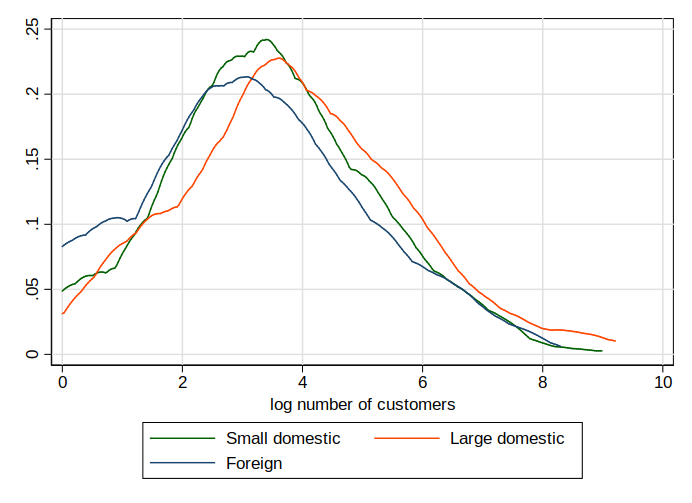
\includegraphics[scale=0.5]{graphs/Fig5a.png}}
    \end{subfloat}
    \begin{subfloat}[By country]
    {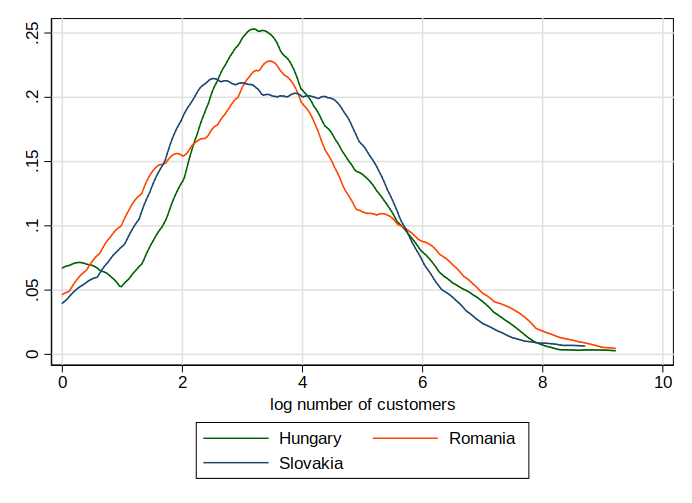
\includegraphics[scale=0.5]{graphs/Fig5b.png}}
    \end{subfloat}
    \end{center}
    {\footnotesize \textit{Notes:} This Figure shows kernel densities of the ln number of customers. Small: $< 51$ employees, large otherwise. Foreign: foreign controlled}     
\end{figure}





The fourth column of Table \ref{tab:num_supp} shows the median share of returning partners ("had bought from /sold to your company previously?")  in all partners. Repeated or longer term relationships seem to be the norm rather than the exception for these firms. In Hungary, for example, for a typical firm, two thirds of buyers and returning buyers while more than 80\% of suppliers supplied the firm previously. We also find that manufacturing firms' relationships with their suppliers are slighly more likely to be repeated than their relationship with their buyers.


The fifth column of Table \ref{tab:num_supp} shows that supplier and buyer protfolios of manufacturing firms are quite concentrated. The largest 3 partners represent between 40-60 percent of sales/purchases for the typical firm. This concentration is high when compared to the typical number of partners. We do not find pronounced differences between the concentration of buyers and suppliers, and these shares are similar across countries.

Finally, the last column of Table \ref{tab:num_supp} shows the length of key relationships. Note that this can be only measured for the key relationships of the most important partners rather than all realtionships. We find that key relationships tend to to relativelly old, between 6 and 10 years for the median firm. The longevity of key supplier and buyer relationships appear to be similar. There are pronounced country differences in this respect, with relationships being about 3 years longer in Hungary compared to the other two countries. 

While Table \ref{tab:num_supp} has shown the central tendencies of the different variables, the survey data also allows us to analyse firm heterogeneity in these dimensions. Figure \ref{fig:happy_few} shows the (inverse) CDFs of the different varaibles. Panel A shows the distribution in the number of customers. In line with the patterns in Figure \ref{fig:kernel}, the distribution is skewed, the median firm having 30 customers and the 99th percentile being 400.

There are also substantial differences across firms in terms of the share of their new (non-returning) customers. 40\% of firms served only returning customers in 2015, while 20\% of firms had a share of new customers above 50\%. This pattern reinforces our earlier conclusion that longer-term relationships are the rule rather than the exceptions, but it also details the picture by showing that different firms face large differences in the share of their longer-term relationships.

The different strategic situation of firms is even more pronounced when we consider the concentration of their buyers. The TOP3 customers of the medium firm are responsible for about half of the sales, but the share of TOP 3 buyers is above 80\% for 20\% of firms. This suggests that most firms face at least some buyers with a large power, but a substantial share of firms depend strongly on decisions of a few firms.

\newgeometry{top=4cm}
\begin{figure}[!h]
    \caption{Differences between firms}
    \label{fig:happy_few}
    \begin{center}
    \subfloat[Number of customers]{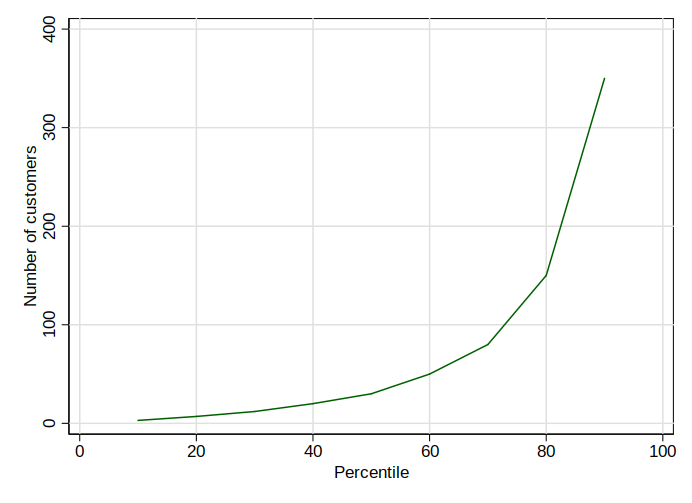
\includegraphics[width=7cm]{graphs/Fig4a.png}}
    \subfloat[Share of new customers]{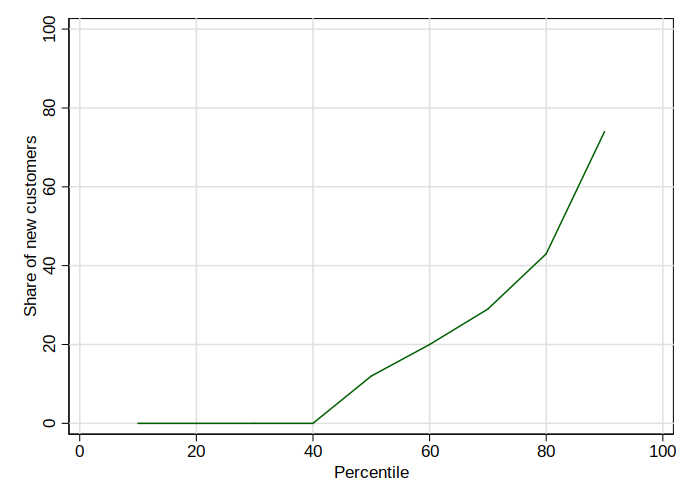
\includegraphics[width=7cm]{graphs/Fig4b.png}}\\
    \subfloat[Share of top customer]{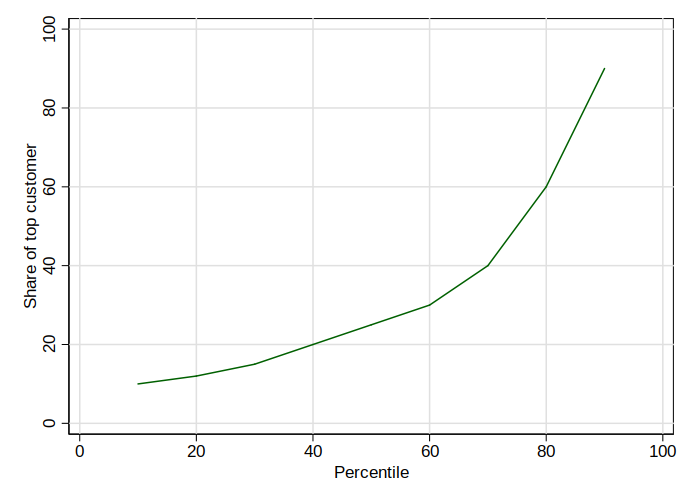
\includegraphics[width=7cm]{graphs/Fig4c.png}}
    \subfloat[Share of top3 customers]{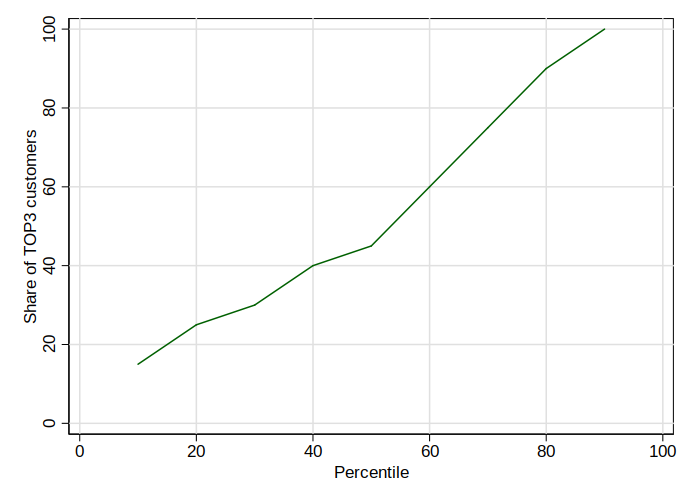
\includegraphics[width=7cm]{graphs/Fig4d.png}}
    \end{center}    
        {\footnotesize \textit{Notes:} This Figure shows the percentages (1-99) of the distribution of the above variables.} 
\end{figure}
\restoregeometry

To sum up, we find that the supplier-buyer relationships of the manufacturing firms in our sample are far away from being atomized and short-term. A large share of partners are returning and the length of key relationships can easily be above 8-10 years. Buyer and supplier power seem to be substantial, with the top 3 partners typically responsible for more than half of sales or purchases. The survey also shows that there is a substantial amount of heterogeneity across firms in terms of how long-term their relationships are and how concentrated their buyer and supplier porfolio is. These facts imply that building supplier/buyer relationships are important strategic choices and may be strongly related to competitiveness.


\subsection{Supplier and buyer portfolios and performance}

In this subsection we coduct a simple analysis to see whether the quantity and quality of suppliers is associated with firm performance. 

To do so, we run regressions at the firm level with labor productivity as the dependent variable and measures of the buyer/supplier portfolio as explanatory variables. In particular, we run the following regression

\begin{equation}
    LP_{i|cjs}=\beta' X_{i}+\gamma \ln employees_i+\eta_c+\theta_j+\delta_s+u_i
\end{equation}{}

where $i$ denotes firms, $c$ countries, $j$ 2-digit industries and $s$ size categories. $X_{i}$ is the vector of the variables of interest, and $\eta_c$, $\gamma_j$ and $\delta_s$ are sets of country, industry and size category dummies. 

This strategy identifies from comparing firms in the same country, industry and size category but with different buyer and supplier structure. Naturally, in this cross sectional regression many key firm variables remain unobserved, therefore the results should be interpreted as suggestive correlations rather than causal effects.

Table \ref{tab:prod_regs} presents the results of these regressions. In columns (1) only the dummies and the number of byuers/suppliers are included. We find that the number of suppliers (but not that of buyers) is strongly correlated with labour productivity. A firm having twice as many suppliers will have 5.6 log points higher productivity levels. 

In column (2) we start to control for the type of partners a firm has. First, we ask whether having at least one buyer and/or supplier from the firm's business group matters for productivity. Indeed, we find a strong relationship between productivity and the presence of \textit{buyers} from the business group: firms having at least one such buyer have a 15 log points higher productivity level. We also investigate in column (2) whether having foriegn buyers or sellers matters for productivity and find no evidence form that. In column (3) we also include the average lenght of the relationship with key buyers and suppliers. These variables are not significant.

To sum up, labor producivity is indeed correlated with the number of suppliers a firm has and also whether some of the buyers are from the same business group. There results underline that partner portfolios are related to performance and therefore being more successful in building such portfolios may generate a competitive advantage,

%% can control for whether the firm is a member of a business group?
\begin{table}[H]
    \caption{Labor productivity and supplier/buyer charateristics}
    \label{tab:prod_regs}
    \centerline{
\begin{tabular}{lccc} \hline
 & (1) & (2) & (3) \\
VARIABLES & LP & LP & LP \\ \hline
 &  &  &  \\
ln(Number of buyers) & 0.014 & 0.021 & 0.016 \\
 & (0.013) & (0.014) & (0.015) \\
ln(Number of suppliers) & 0.059*** & 0.057*** & 0.069*** \\
 & (0.017) & (0.017) & (0.019) \\
Has buyer from business group &  & 0.137** & 0.155** \\
 &  & (0.057) & (0.061) \\
Has supplier from business group &  & -0.073 & -0.050 \\
 &  & (0.060) & (0.064) \\
Has foreign buyer &  & 0.023 & 0.035 \\
 &  & (0.051) & (0.057) \\
Has foreign supplier &  & -0.081 & -0.056 \\
 &  & (0.050) & (0.058) \\
Mean relationship length, buyers &  &  & 0.007 \\
 &  &  & (0.005) \\
Mean relationship length, sellers &  &  & -0.005 \\
 &  &  & (0.005) \\
ln(Employment) & 0.110*** & 0.104*** & 0.097*** \\
 & (0.025) & (0.026) & (0.028) \\
Group member & 0.161*** & 0.140*** & 0.136** \\
 & (0.049) & (0.052) & (0.057) \\
\hline
Country, sector, size dummies &YES &YES &YES\\
Observations & 1,129 & 1,129 & 996 \\
 R-squared & 0.325 & 0.330 & 0.339 \\ \hline
\end{tabular}

}
    {\scriptsize \textit{Notes:} The table shows OLS regressions when the dependent variable is ln(labor productivity). One observation is one respon- dent. Business group and for- eign refers to whether the firm has at least one such partner, while length is the average length of key relationships. Standard errors in parentheses$ *** p$<$0.01, ** p$<$0.05, * p$<$0.1 $}
\end{table}
    



\subsection{Starting relationships}

After showing that performance is related to the number and type of buyers of the firm, it fundamental to ask how these relationships form, i.e. what firm can and should do to build a portfolio which can support high performance more effectivelly.

\subsubsection{How relationships form}

In our questionnaire we asked about each key relationship how it was formed. Based on the answer to that question we can distinguish between (i) supplier initiated; (ii) buyer initiated; (iii) within groups and (iv) Other ways (including professional events). 



Buyer and supplier-initiated relationships are similarly important. Network etc is relatively less important\\
By country:

\begin{figure}[h]    
    \begin{center}
    \label{fig:rel_form}    
    \caption{How do firms find customers?}  
    \begin{subfloat}[By country]
    {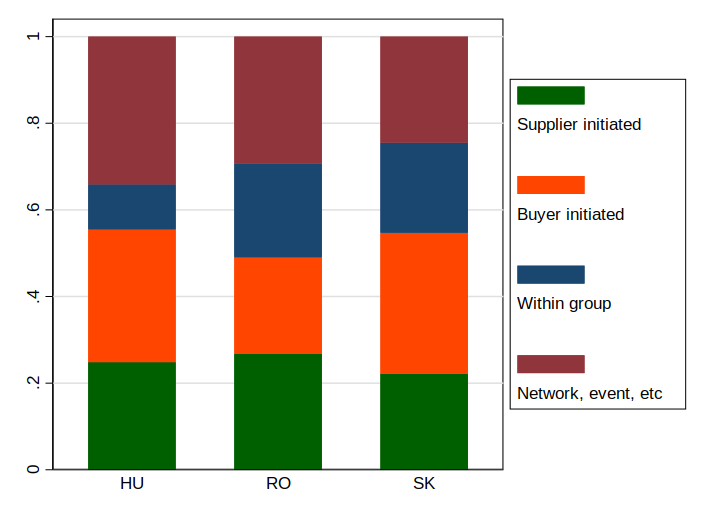
\includegraphics[scale=0.5]{graphs/Table6a.png}}
    \end{subfloat}
    \begin{subfloat}[By firm type]
    {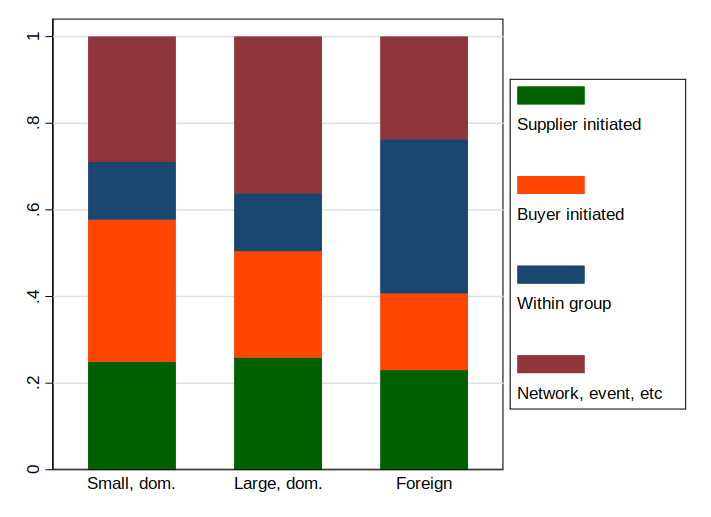
\includegraphics[scale=0.5]{graphs/Table6b.png}}
    \end{subfloat}
    \end{center}
    {\footnotesize \textit{Notes:} The figure shows the distribution of the answers to ’how the relationship started?’ for key relationships (each such relationship when respondent is supplier is one observation).}     
\end{figure}


%%%PUT these two figures into one please!

\subsubsection{Innovation}

\begin{itemize}
    \item Significant part of supplier relationships starts with innovation. Product and process innovation are complementary. Large country differences.
  

    
 \begin{figure}[h]    
    \begin{center}
    \label{fig:inn}    
    \caption{Innovation when relationship starts}  
     \label{fig:innov}
    \begin{subfloat}[By country]
    {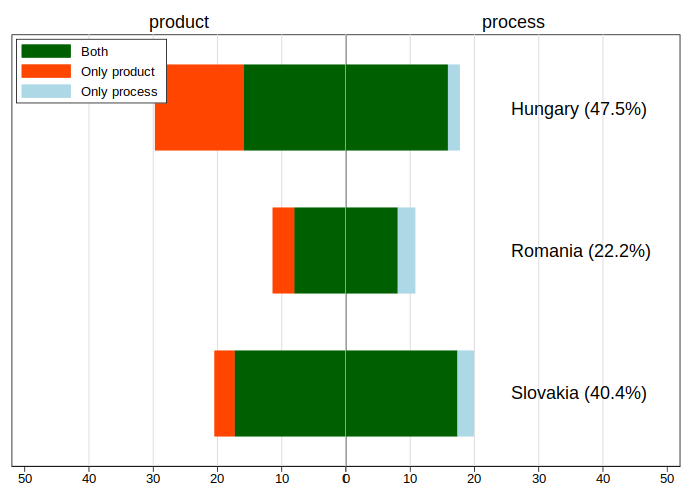
\includegraphics[scale=0.5]{graphs/Fig7a.png}}
    \end{subfloat}
    \begin{subfloat}[By size and ownership]
    {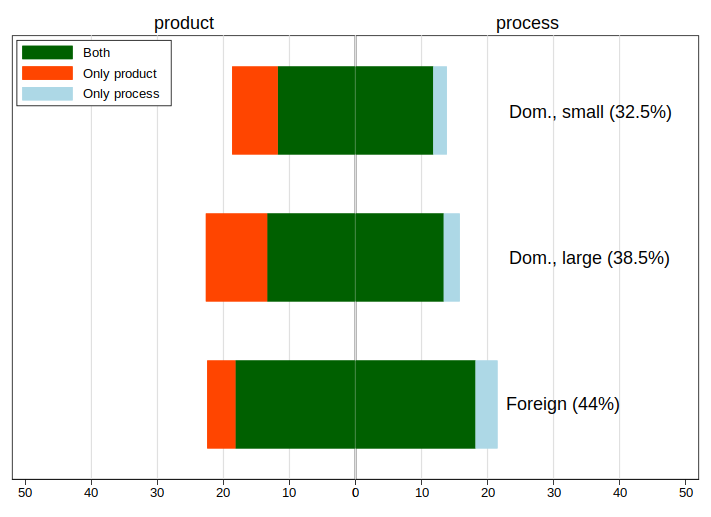
\includegraphics[scale=0.5]{graphs/Fig7b.png}}
    \end{subfloat}
    \end{center}
    {\footnotesize \textit{Notes:} The figure shows the distribution of the answers to ’did the firm have to improve its product/process for the relationship at the beginning’ for key relationships (each such relationship when respondent is supplier is one observation).}     
\end{figure}   
    

    \item Buyers, especially domestic ones, often provide assistance for product development: consulting in 1/4, technology transfer in 1/8 and asset transfer in 1/16 of key relationships.
\end{itemize}
    
\begin{table}[h]
    \caption{Firm characteritics and relationship lenght (median)}
    \label{tab:char_length}    
    
\begin{tabular}{lcccc} \hline
Partner (buyer) &	\multicolumn{4}{c}{Respondent (seller)}	\\		
	&Domestic SME	&Domestic large	&Foreign-owned	&Total\\
	\hline
	\hline
&\multicolumn{4}{c}{Technology transfer}\\
Domestic SME&	16.2&	100.0&	63.6&	19.2\\
Domestic large&	24.1&	27.8&	25.7&	24.6\\
Abroad&	12.0&	25.7&	13.8&	12.5\\
Total&	15.3&	27.8&	24.6&	16.4\\
\hline
&\multicolumn{4}{c}{Asset transfer}\\
Domestic SME&	7.9&	0.0&	63.6&	10.5\\
Domestic large&	14.7&	11.1&	17.0&	14.9\\
Abroad&	3.2&	8.6&	12.1&	3.6\\
Total&	6.4&	9.5&	17.9&	7.3\\
\hline
&\multicolumn{4}{c}{Regular meetings, consulting}\\
Domestic SME&	22.2&	50.0&	54.5&	24.0\\
Domestic large&	34.0&	31.5&	33.3&	33.8\\
Abroad&	18.8&	25.7&	25.9&	19.2\\
Total&	22.8&	28.6&	32.5&	23.7\\
\hline
\end{tabular}

    {\scriptsize \textit{Notes:} The figure shows the median length of key relationships (each such relationship when respondent is supplier is one observation). SME: <=50 employees, large otherwise.}
\end{table}


\begin{table}[h]
    \caption{Support for innovation from customers at the start of the relationship}
    \label{tab:start_support}
    
\begin{tabular}{lcccc} \hline
Type of customer	&\multicolumn{4}{c}{Type of reporting firm (seller)}	\\		
	&Domestic SME	&Domestic large	&Foreign-owned	&Total \\
	\hline
	\hline
&\multicolumn{4}{c}{Technology transfer}\\
Domestic SME	&18.1	&100.0	&63.6	&21.0 \\
Domestic large	&25.2	&25.9	&25.7	&25.3
Abroad	&13.0	&27.1	&20.7	&13.7\\
Total	&16.4	&27.8	&26.2	&17.5\\
\hline	
	
&\multicolumn{4}{c}{Asset transfer}\\
Domestic SME&	6.9&	0.0&	63.6&	9.6\\
Domestic large&	15.0&	11.1&	15.8&	14.9\\
Abroad&	4.2&	8.6&	10.3&	4.5\\
Total&	7.1&	9.5&	16.7&	7.8\\
\hline
&\multicolumn{4}{c}{Regular meetings, consulting}\\
Domestic SME&	24.5&	50.0&	54.5&	26.2\\
Domestic large&	39.0&	27.8&	34.5&	37.6\\
Abroad&	23.9&	31.4&	29.3&	24.3\\
Total&	27.7&	30.2&	34.2&	28.2\\
\hline
\end{tabular}


    {\scriptsize \textit{Notes:} The figure shows the distribution of the answers to the question about the type of assistance provided by the buyer for product development at the start of the relationship for key relationships (each such relationship when respondent is supplier is one observation). SME: $<50$ employees, large otherwise.}
\end{table}



\section{Summary and discussion}


% todo miklos. what we learnt. what this data can be used for. what are the questions for which such data is needed. debates in econ vs policy? 


\section{References}

\bibliographystyle{agsm}
\bibliography{biblio}

\appendix
\section{Appendix}

\end{document}
